\documentclass[class=report, crop=false, 12pt,a4paper]{standalone}
\usepackage{enumitem}
\usepackage{multicol}
\usepackage{graphicx}
\usepackage{float}
\usepackage{amsmath}
\usepackage{amssymb}
\usepackage{mathtools}
\usepackage{siunitx}
\usepackage{commath}
\usepackage{array}
\usepackage{natbib}
\usepackage[a4paper,width=150mm,top=25mm,bottom=25mm]{geometry}
\setlength{\parindent}{0pt}
\begin{document}
\chapter{Public Goods and Externalities}
\section{Introduction}
\subsection{Aims}
\begin{enumerate}
	\item Recall the two dimensions of public good (rivalry and excludability) and understand how they lead to market failure
	\item Identify and describe the occurence and results of positive and negative externalities
	\item Understand the role of the public sector in managing market failures arising from public goods and externalities
	\item Be aware of the particular challenges related to climate externalities
	\item Become familiar with the dimensions of the environmental ceiling and social foundations of the doughnut economic model
\end{enumerate}
\subsection{Market equilbirium}
Market equilibirium occurs when supply equals demand. Private marginal benefit of consumption is equal to private marginal cost of production.
\begin{figure}[H]
	\centering
	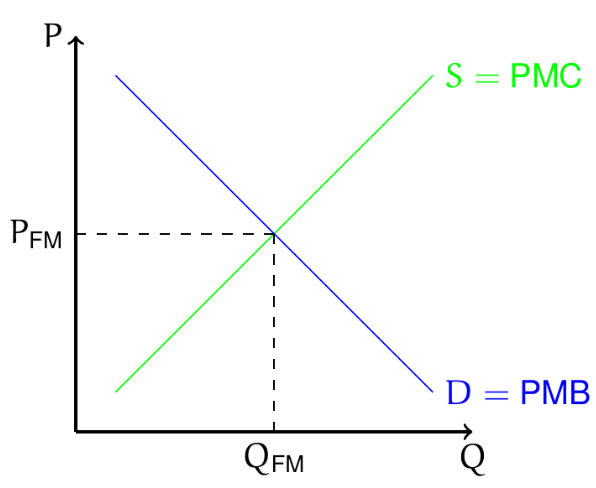
\includegraphics[width = 0.5\textwidth]{../img/figure13.png}
	\caption{Market equilibrium.}
\end{figure}
\subsection{Public goods and externalities}
\subsubsection{Definitions}
Public goods:
\begin{quote}
	Goods which are both non-excludable and have non rivalrous consumption.
\end{quote}
Externalities:
\begin{quote}
	Positive or negative effects on third parties arising from the production or consumption of goods, that are not reflected in the price
\end{quote}
\subsubsection{Market failures}
Public goods and externalities cause market failures in the allocation of goods/services at the free-market equilbirium.
\begin{itemize}
	\item i.e. $Q_{\textrm{free-market}}$ is not optimal
	\item addressed through the allocative role of government
\end{itemize}
\section{Public goods}
\subsection{Two dimensions of public good}
\textbf{Excludability:} the degree to which access to a good, service or resource can be restricted.
\begin{itemize}
	\item \textbf{Excludable:} agents can easily be prevents from using the good/service
	\item \textbf{Non-excludable:} preventing agents from consuming the good/service is impossible (or very expensive)
\end{itemize}
\textbf{Rivalry:} the degree of which consumption by one party affects another parties use of the good.
\begin{itemize}
	\item \textbf{Rivalrous:} consumption by one agent prevents simultaneous consumption by other agents, or reduces the marginal benefit of another agents
	\item \textbf{Non-rivalrous:} once it is provided, the additional resource cost of another person consuming the good is zero (i.e. MC = 0) and the marginal benefit does not decrease with number of users
	\item (\textbf{Anti-rivalrous:} marginal benefit increases with the number of users, e.g. social network)
\end{itemize}
\subsection{Rivalry and capacity}
Goods are often non-rivalrous up to a certain capacity, above which they are rivalrous e.g. public transport (bus/train), road bridge, internet bandwith.
\subsection{Continuous scale}
\begin{figure}[H]
	\centering
	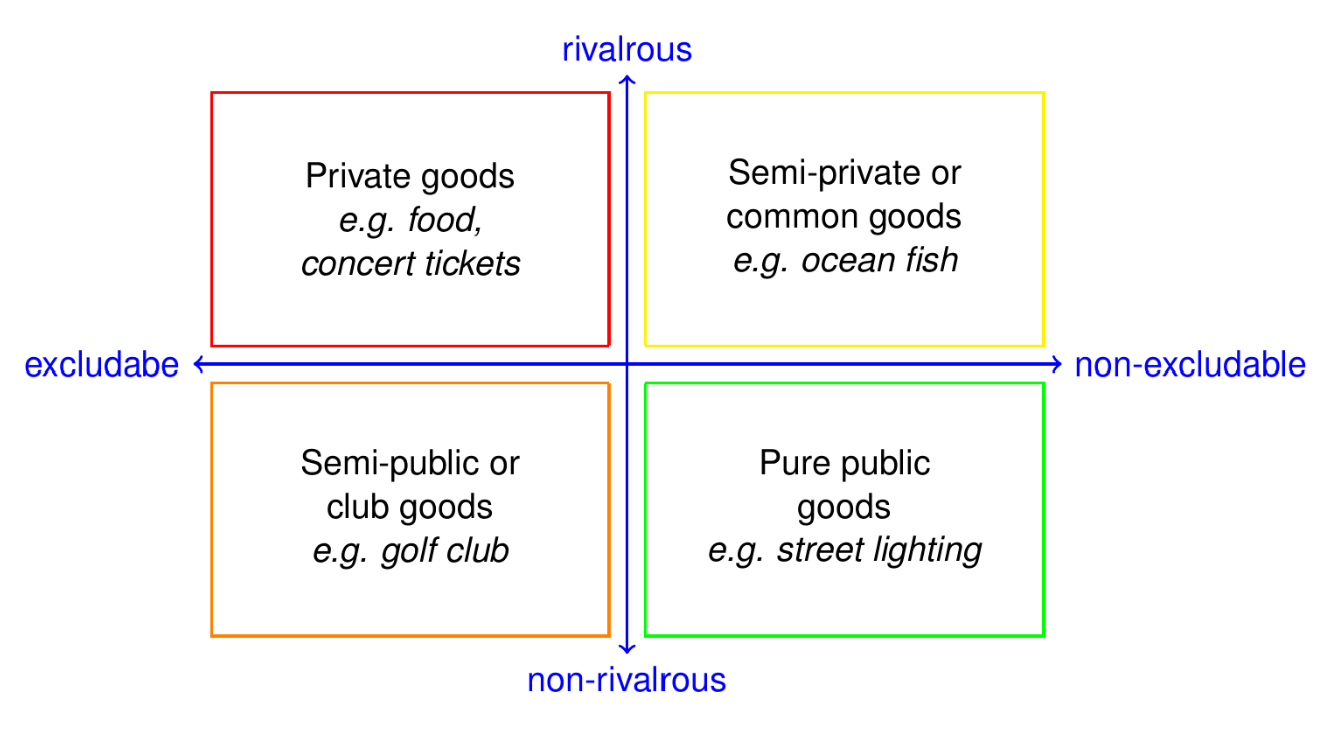
\includegraphics[width = \textwidth]{../img/figure14.png}
	\caption{Continuous scale.}
\end{figure}
\subsection{Public goods in free markets}
\begin{figure}[H]
	\centering
	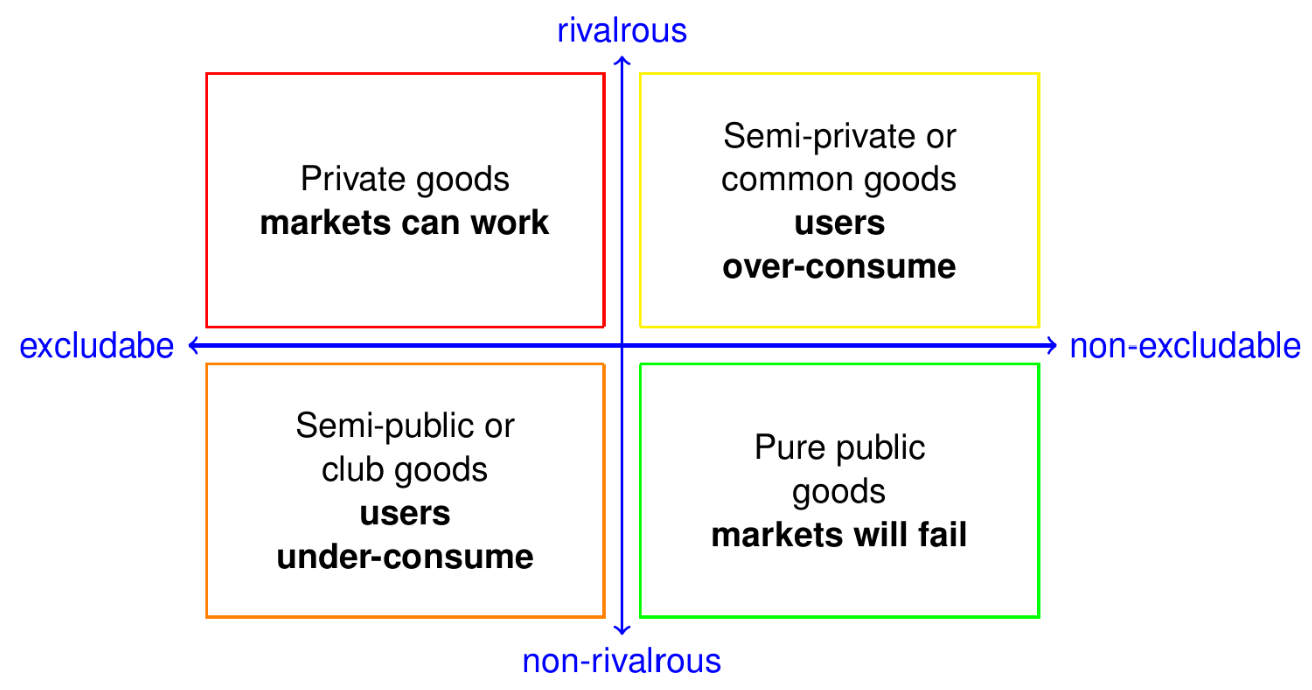
\includegraphics[width = \textwidth]{../img/figure15.png}
	\caption{Public goods in free markets.}
\end{figure}
\subsection{Public goods and market failure}
Pure public goods are \textbf{non-excludable}
\begin{itemize}
	\item Producers cannot exclude agents from consumption
	\item Unable to charge and therefore make profit
	\item Therefore (in theory) would not be produced through market action!
\end{itemize}
Possibility of funding via private cooperative, but\dots

\textbf{Free rider problem}
\begin{quote}
	as size of cooperative increases, possibility of avoiding contributing increases
\end{quote}
\subsubsection{Public sector provision}
Large group public goods supplied from public sector budget
\begin{itemize}
	\item Allocative role of government
\end{itemize}
\subsection{Privatisation in the public sector}
Note\dots Public sector provision $\neq$ equivalent public sector production.
\begin{quote}
	The creation of markets in public services has been one of the great defining shifts in the way government has been run over the past 30 years (Gash and Roos 2012)
\end{quote}
\section{Externalities}
\subsection{Positive and negative externalities}
Externalities
\begin{quote}
	when the actions of one economic agent directly affect other agent(s) outside the market mechanism (production/consumption)
\end{quote}
Externalities can arise from either production or consumption and have a net positive or negative effect. 
\subsection{Negative production externality}
\begin{figure}[H]
	\centering
	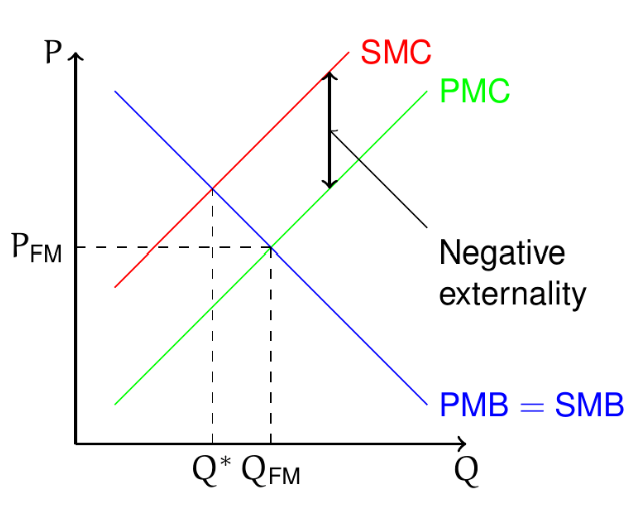
\includegraphics[width = 0.5\textwidth]{../img/figure16.png}
	\caption{Negative production externality.}
\end{figure}
Production of output reduces well-being of third parties not involved in transaction, 
\begin{itemize}
	\item e.g. oil spills during fuel production pollute oceans and damage wildlife
	\item leads to overproduction
\end{itemize}
\subsection{Negative consumption externality}
\begin{figure}[H]
	\centering
	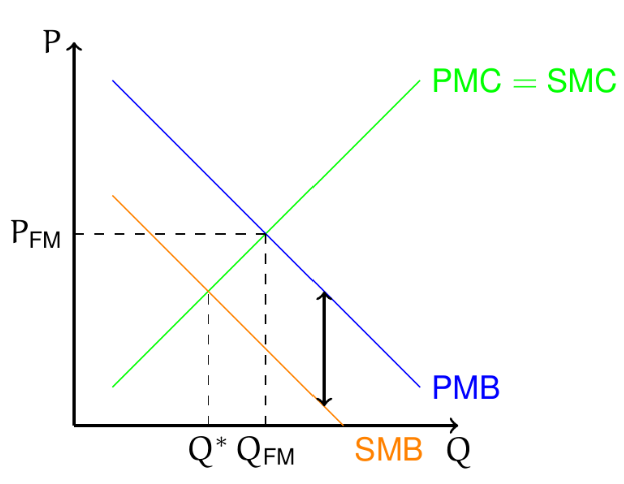
\includegraphics[width = 0.5\textwidth]{../img/figure17.png}
	\caption{Negative consumption externality.}
\end{figure}
Consumption of output reduces well-being of third parties not involved in transaction,
\begin{itemize}
	\item e.g. driving cars produces carbon emissions
	\item leads to overconsumption
\end{itemize}
\subsection{Positive production externality}
\begin{figure}[H]
	\centering
	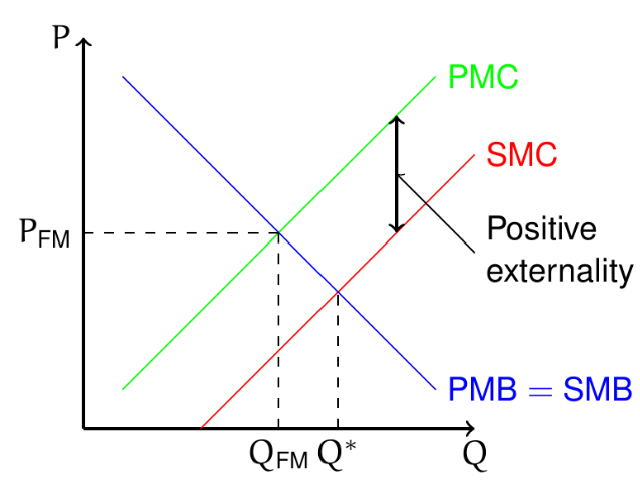
\includegraphics[width = 0.5\textwidth]{../img/figure18.png}
	\caption{Positive production externality.}
\end{figure}
Production of output reduces well-being of third parties not involved in transaction,
\begin{itemize}
	\item e.g. creating a new tourist attraction brings increases custom to local shops
	\item leads to underproduction
\end{itemize}
\subsection{Positive consumption externality}
\begin{figure}[H]
	\centering
	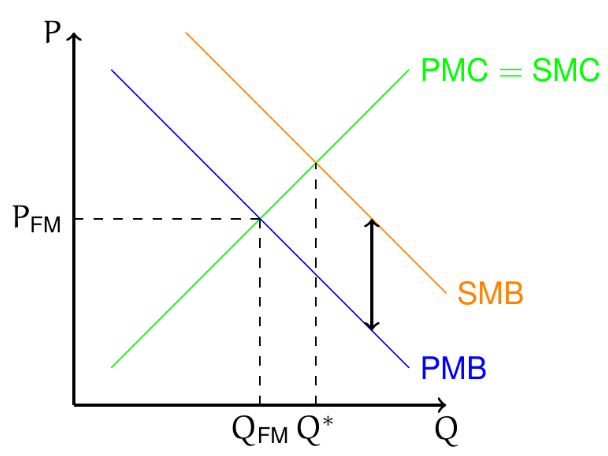
\includegraphics[width = 0.5\textwidth]{../img/figure19.png}
	\caption{Positive consumption externality.}
\end{figure}
Consumption of output reduces well-being of third parties not involved in transaction,
\begin{itemize}
	\item e.g. cycling improves peoples general health, rducing pressure on public healthcare
	\item leads to underconsumption
\end{itemize}
\subsection{Externalities and property rights}
Externalities can be transferred where third party benefit/cost is clear i.e. where property rights are well defined.
\subsection{Managing externalities}
Where property rights are not clear, managing externalities relies on allocative role of government
\subsubsection{Public sector interventions}
Negative externalities:
\begin{itemize}
	\item Corrective taxes
	\item Quantity restrictions
	\item Standards
\end{itemize}
Positive externalities
\begin{itemize}
	\item Subsidies
	\item Tax benefits
	\item Direct production
\end{itemize}
\subsection{Externalities and the environment}
Note\dots Externalities related to climate change are critical to long term sustainability of the planet.
\subsubsection{COP26}
\begin{quote}
	``Climate change is the single benefit health treat facing humanity. While no one is safe from the health impacts of climate change, they are disproportionality felt by the most vulnerable and disadvantaged.'' (World Health Organisation 2021)
\end{quote}
\subsection{The doughnut economic model}
\begin{figure}[H]
	\centering
	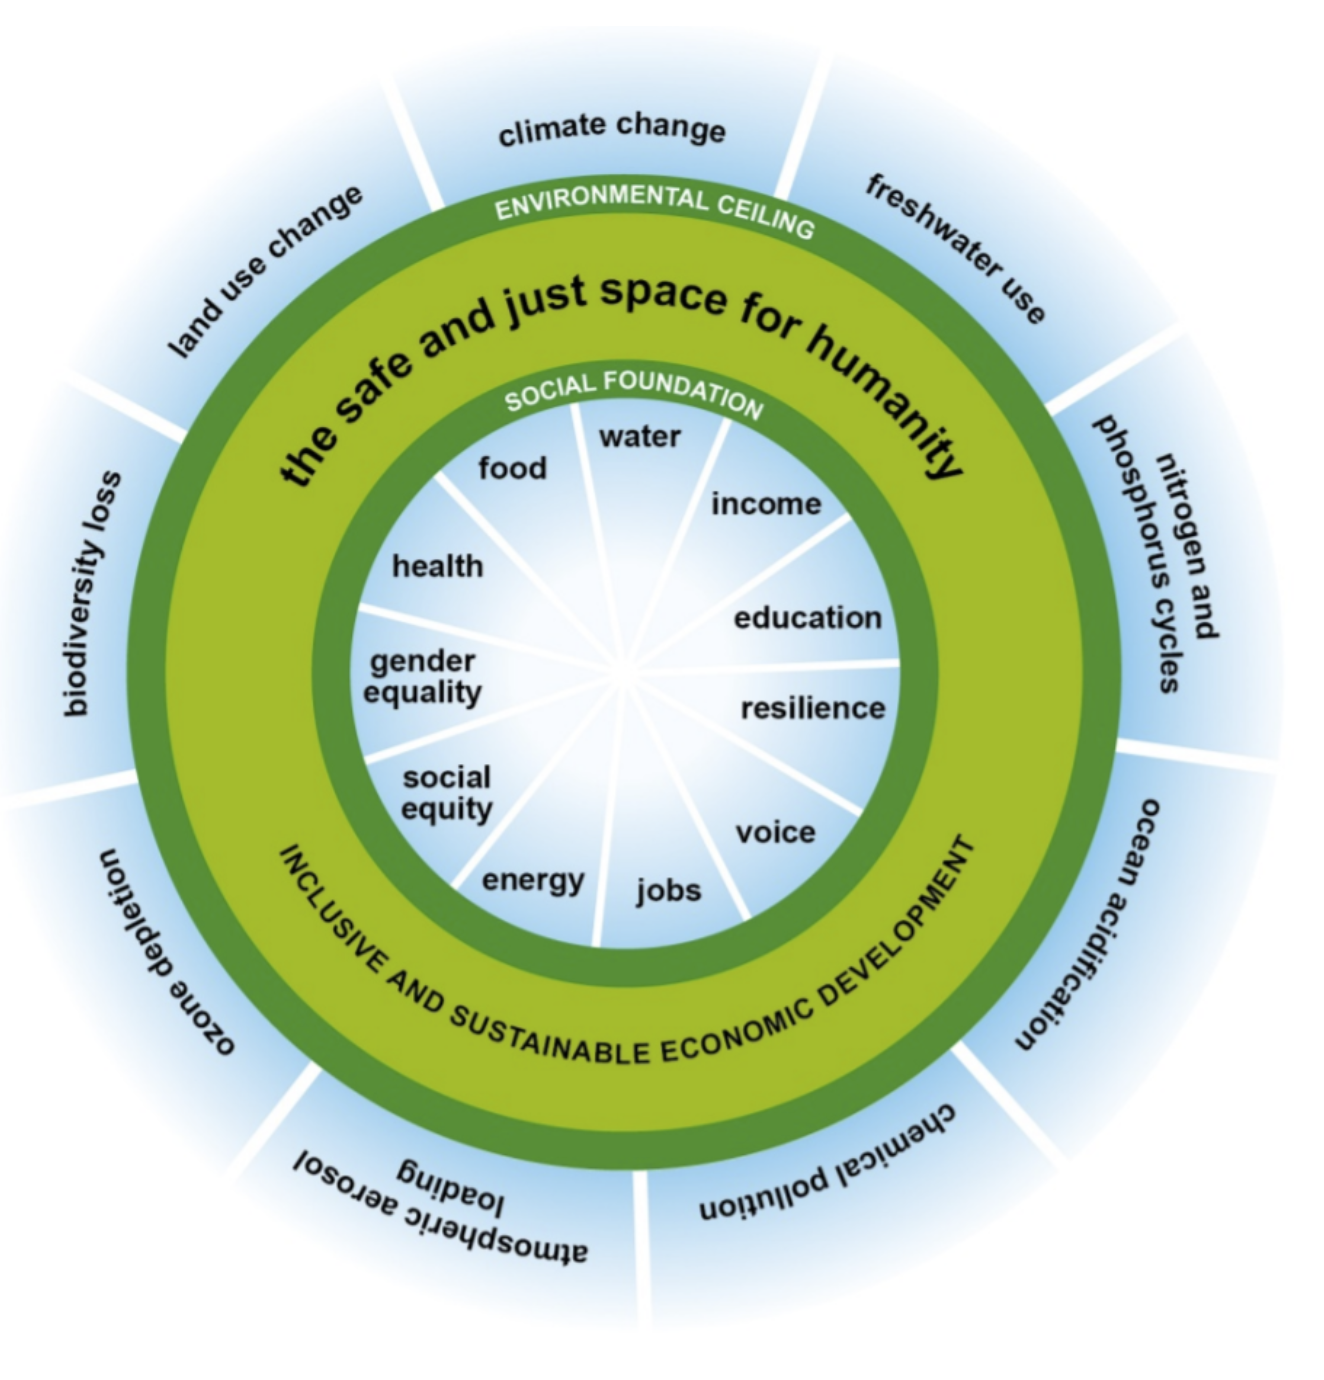
\includegraphics[width = \textwidth]{../img/figure20.png}
	\caption{Doughnut economic model.}
\end{figure}
\end{document}